\chapter{Introduction}
\label{ch:introduction}
\section{Motivation}

Since the advent of modern digital communications in the 20th century, there has been an explosion in the demand for wireless spectrum. As a result, spectrum is becoming an increasingly scare resource. This demand is a direct result of the availability and relatively inexpensive cost of such wireless devices. Therefore, in such environments as military operations, disaster relief scenarios, and natural defense situations, the probability of interfering transmissions \cite{scarcity}, intended and unintended, has steadily grown to a point where techniques are needed in-order to combat such occurrences. More directly, in such situations when interfering signals are partially or completely understood measures need to be devised in-order to overcome such difficulties.

%Since the advent of modern digital communications in the 20th century there has been an explosion in the demand for wireless spectrum.  As a result spectrum is becoming an increasingly scare resource\cite{scarcity}.  This demand is a direct result of the availability and relatively inexpensive cost of such wireless device.  Therefore in such environments as militaristic theatres the probability of interfering transmissions, intended and unintended, has steadily grown to a point where techniques need to be consider to combat such occurrences.  More directly, in such situations when interfering signals are partially or completely understood measures can be taken to overcome such difficulties.\\


In military theatres, it is extremely common to observe friendly operated high-power broadband jamming signals \cite{frater}.  Such devices exists as part of group convoys in several branches of the military and in many other forms across a variety of deployments.  Unfortunately, such devices block both friendly and hostile communications, and current anti-jamming techniques have not provided a viable solution to this problem.  Therefore, new approaches should be considered, utilizing more flexible radio technologies.\\

Understanding how to overcome such challenges is a complex task; with vastly different transmission environments and differing operating devices and operating standards.  A new system that could combat such pitfalls should rely on all friendly information, or be able to construct solutions of its own from a set of tools given to the radio.  Such tools should be flexible and easily modified, changed, or improved.  This ability to easily change or adapt is a key feature as the technical requirements can change from day to day, or between branches of the military itself. As such a solution should have the following attributes:

\begin{itemize}
\item \textbf{Flexible:} Easily adaptable to many situations and interference types, while still relying on the same hardware.

\item \textbf{Efficient:} Relatively low hardware cost and low computational complexity

\item \textbf{Robust:} Designed to provide guaranteed performance gains even under severe channel conditions

\end{itemize}


\section{State of the Art}

Current implementations of anti-jamming technology lies on the straddling point of hardware and software in the communications world.  This is true because hardware provides the speed and performance needed for digital data transmission, while software provides higher level intelligence and flexibility in such layers as the media access control layer and the network layer of the Open Systems Interconnect (OSI) model \cite{Zimmermann}.  An outline of the model can be seen in Figure \ref{osi_model}. For anti-jamming applications, smarter radios allow for enhanced mobility against the jammer.  Therefore, a largely focused software implementation, allowing for highly intelligent radio decisions, must be considered when investigating anti-jamming techniques.\\

\begin{figure}[!ht]\label{osi_model}
\centering
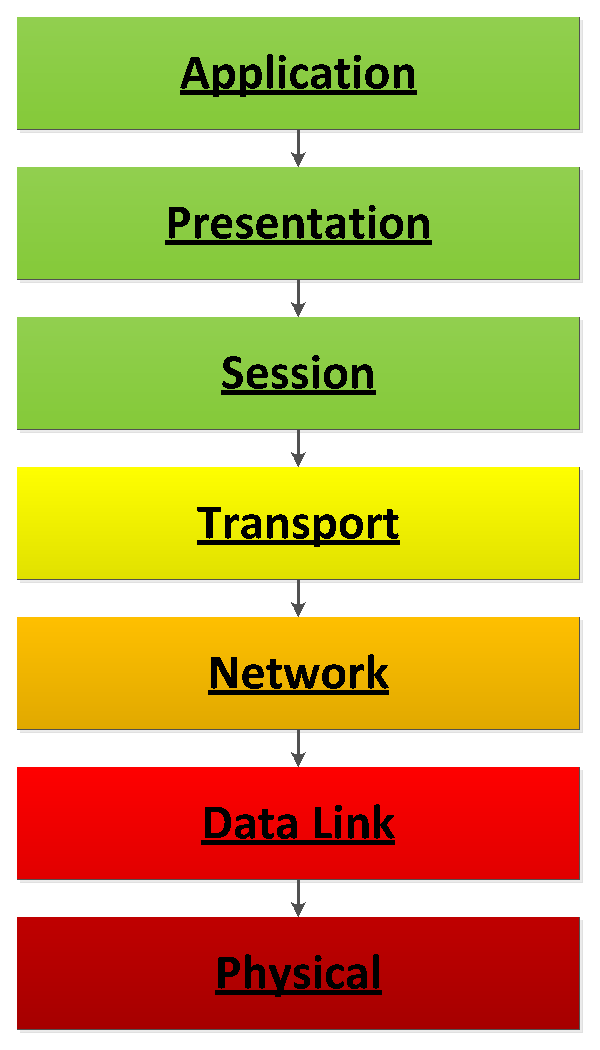
\includegraphics[scale=0.50]{OSI_model.eps}
\caption{The Open Systems Interconnection model is made up of 7 layers, but three primary sections.  This thesis primarily focuses on the lowest level of this model, the physical layer.}
\end{figure}

Current anti-jamming techniques include channel hopping, spatial retreat, jammed area mapping, node escape, retreat restoration, frame masking, and many more \cite{1}.  All of these techniques use mechanisms of evasion or deception.  These can be quite effective when attacked by generally narrowband, non-dynamic/non-learning jammers.  In the case of wide and ultra-wide band jammers, these techniques are not as effective.  This wide-band environment is the primary situation of interest, and it generally considered a technically challenged scenario.  These anti-jam techniques are design for specific situations and jammers.\\

Let us first examine these anti-jamming techniques which are broken down into three primary categories: Proactive countermeasures, Reactive countermeasures, and Mobile agent-base countermeasures \cite{1}.  Reactive countermeasures relies on a varying array of detection mechanisms first to determine if that node is being jammed.  These detection methods  must be coupled with a countermeasure or the scheme is inoperable.  Examples of these detection methods include a transmitter-based approach and a receiver-based detection\cite{detjam}.  In a transmitter-based approach, such as ad-hoc networks, a decision algorithm is used based on four metrics: Packet Delivery Ratio (PDR), Received Signal Strength Indicator (RSSI), Physical rate, and Noise levels \cite{3}.  In the receiver-based detection additional information must be injected into frames to help the receiver determine the number of frames lost.  Since frames can be easily lost in wireless transmissions, the receiver is handicapped when determining the number of retransmissions that have occurred.  In the transmitter the PDR is deterministically determined by the data-link layer, sequence numbers must be added to frames for the receiver to accurately calculate the PDR \cite{3}.  Several other detection methods exist including using a detected detector, cooperative detection among nodes in a wireless network, and more sophisticated methods of RF fingerprinting \cite{3}.\\

Once the jammer has been detected the reactive countermeasures come into play.  Many evasion techniques exists to combat narrowband jammers such as: channel hoping, spatial retreat, retreat restoration, hybrid attacks, and many cognitive radio approaches \cite{2}.  Many of these techniques utilize the network itself to adapt to the jammer, which is an appropriate assumption because without a network wireless communications are irrelevant.  Channel hopping is simple and can be considered straightforward to implement.  If a channel is beginning jammed, a communication system can simply ``hop'' to another channel.  This is easily defeated in two cases: The first case involves the jammer following you or the jammer is simply wide-band capable.  In the second case, one can employ spatial retreat, which is a mechanism to physically evade the areas being jammed. Based on the detection algorithm, all nodes in a network try to estimate the jammed region and flee physically in the direction of safer place. Based on their estimation about the jammed region, nodes will utilize shortest path algorithms to determine location of retreat \cite{5}.  Retreat restoration is focused around how to rebuild a network once the jammer has left.  Retreat restoration can be done by coordinated or uncoordinated communication, and the transmissions are based on a preplanned hop patterns among nodes \cite{6}.\\

There also exists systems that are design to resist jamming pro-actively.  These hybrid systems \cite{7} utilize preventatives measure to resist jamming such as frequency hopping spread spectrum (FHSS).  Spread-spectrum signals are highly resistant to narrowband jamming, unless the jammer has knowledge of the spreading key. In military applications, the spreading key is generally created using a cryptographic function \cite{sterling}.  More hybrid solutions include synchronous and asynchronous spectral multiplexing where intermediary nodes are used to communicate at multiple channels.  When a node changes its channel because of jamming a neighbor will heal that connection by communicating  with the node on its new channel and rest of the network on the old channel \cite{8}.


The largest problem with these techniques is they all have are designed to combat narrowband jammers, and even friendly jammers.  If high powered wideband jammers enter the equation, all of these solutions begin to fall apart.  Note these techniques primarily exploit the dimensionality of their environment by simply avoiding the jammer, and all techniques require intelligent flexible hardware solutions.   To implement such solutions requires sophisticated hardware implementations, that can be quite rigid for rapidly changing communication environments and adversaries.  To compensate solutions that push more of the radio operations from their original rigid hardware implementations into the more flexible software domain, provide a more cost effective and elegant solution.  These software focused radios, also know as software defined radios (SDR), have provided a solid platform for very adaptive anti-jamming technologies under the name cognitive radios \cite{sdr_jam}.  These radios have the ability to easily learn and adapt to their environment, which is the primary requirement of anti-jamming devices.\\

As mentioned above, it is quite common for the military to self-jam its own channels as a result of co-channel interference.  Unfortunately, this can hinder their own use unintentionally.  These disrupted users are known as ``disadvantage users''.  They are commonly small mobile hand-held devices and cannot simply overcome the jammer computationally or in raw power.  Therefore, more manageable and elegant solutions must be considered for such disadvantaged users.  Beside self-jammming, adversarial jammers must also be considered.  Fortunately, certain characteristics can be statistically exploited if these jammer abide by certain properties. Since adversarial jammers tend to inject random data or energy to block communication, if these transmissions can be shown to repeat they can be exploited.  In the case of self-jamming, the signal characteristic can be know \textit{a priori}.  Therefore they also can exploited or removed, negating the effects of such devices.  Such scheme must consider the energy or symbols of the jammmer that are orthogonal and/or non-orthogonal to the symbols of the communication itself.\\


The goal of this project is to exploit a self-jammed and statistically deterministic adversarially jammed channel, through the utilization of cognitive radio, implemented on a software defined radio platform.  Software defined radios, defined as the intersection between hardware radios and computer software \cite{4}, provide a platform flexible enough to support highly intelligence operations such that anti-jamming requires.  A proposed adaptive signal processing software solution for mitigating the effects of both intentional and unintentional jamming (including wideband jamming) via the combination of antenna subset selection, spectral subtraction, and blind source separation (BSS) techniques in order to extract specific transmissions from a mixture of intercepted wireless signals is shown in Figure \ref{bliss_goal}. The goal of our proposed solution, called BLInd Spectrum Separation (BLISS), is to enable reliable, high throughput, and robust end-to-end wireless communications.\\

\begin{figure}[!ht]\label{bliss_goal}
\centering
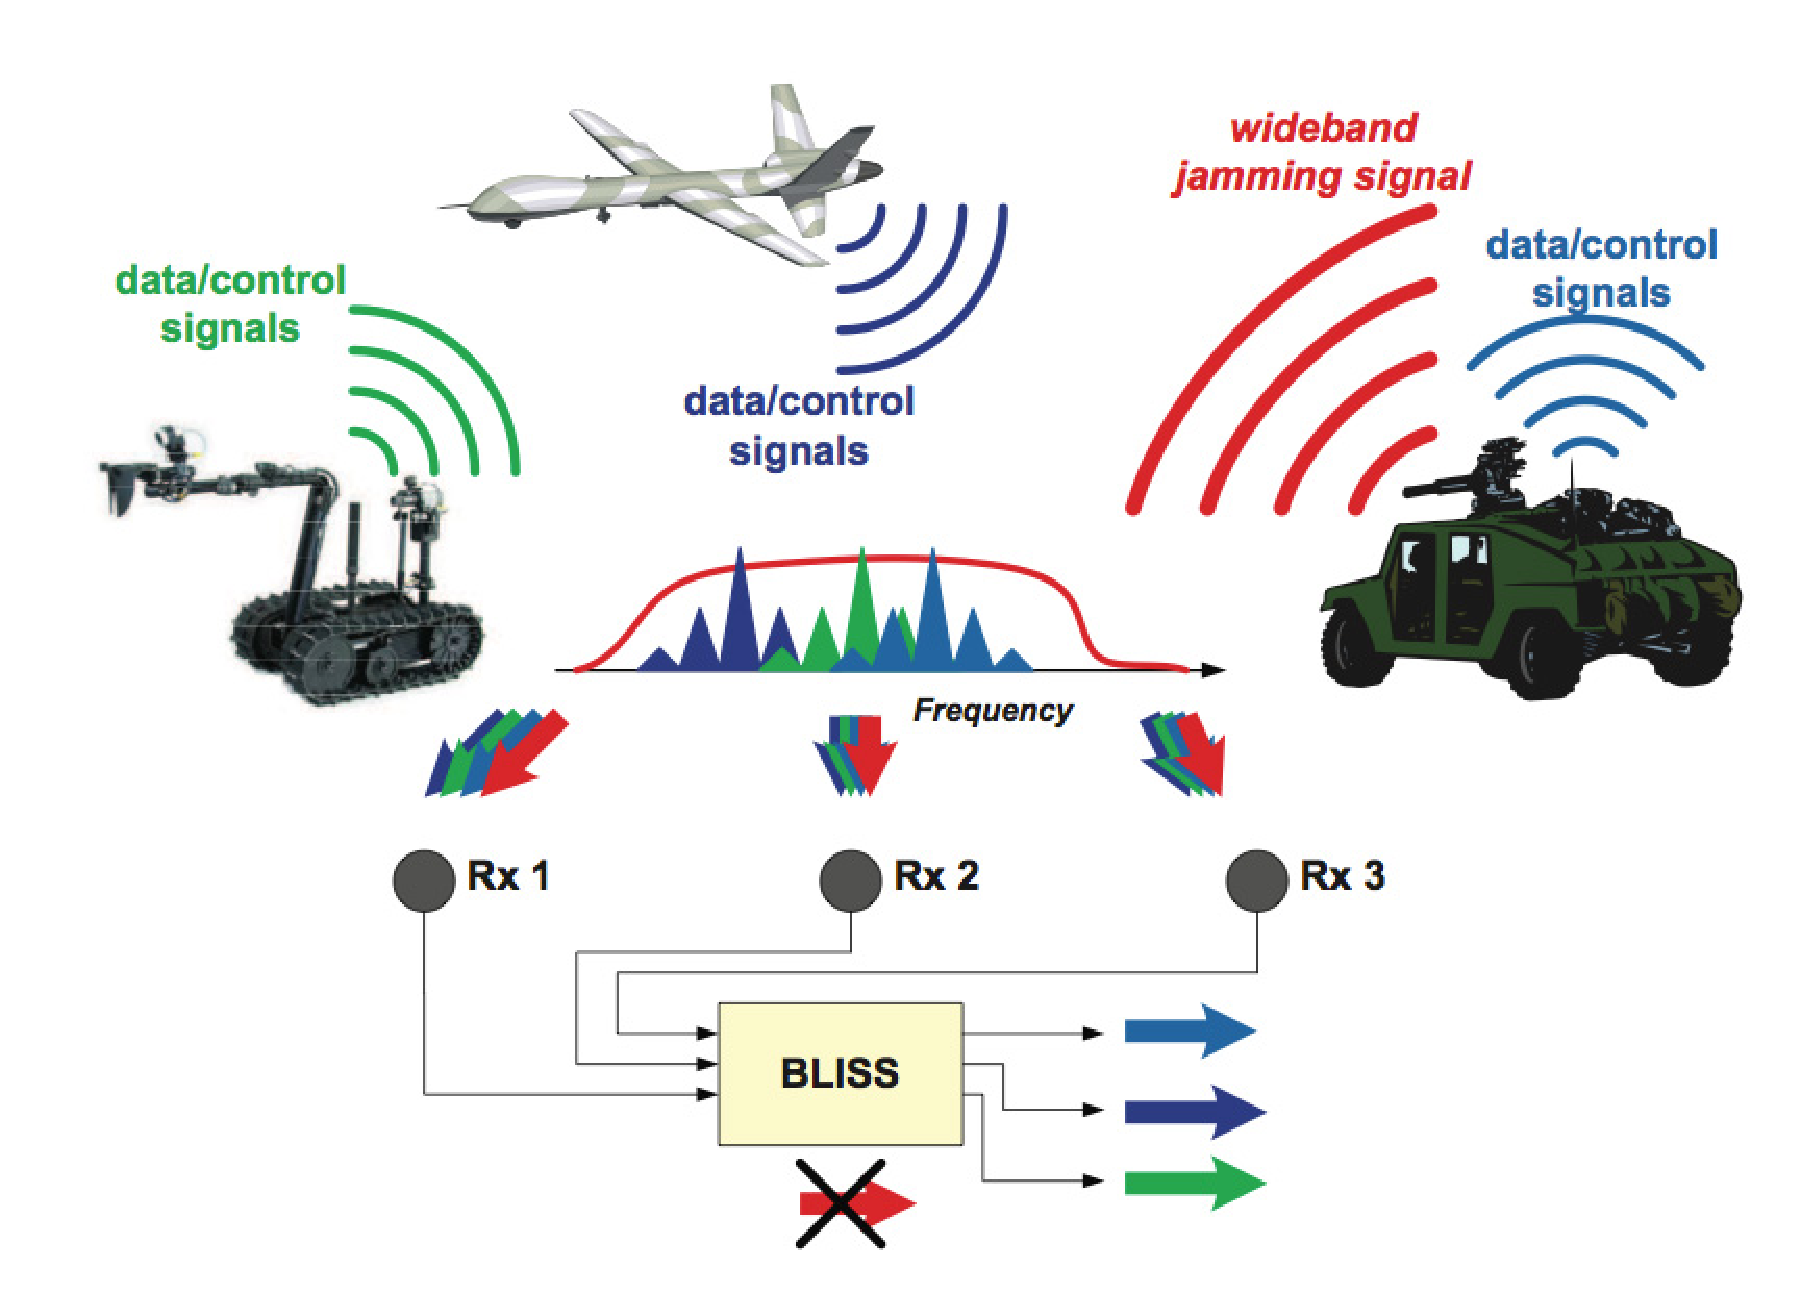
\includegraphics[scale=0.50]{bliss_goal.eps}
\caption{Original system proposed, with the goal of separating desired signals from a spectrally mixed cluster.  This ``BLISS'' system would allow many systems to easily coexist.}
\end{figure}

This work is a continuation of the work done through a collaboration of Worcester Polytechnic Institute and the United States Naval Academy.  Primarily literature surveys and early simulations were completed or attempted before the transition of the project to the work done by this thesis.  Credit is given to the following authors and there coinciding section or block as follows: 

\begin{itemize}
\item \bf{Blind Source Separation:} Dr. Srikanth Pagadarai and Ryan Dobbins 
\item \bf{Spectral Subtraction:} Robert Over
\item \bf{Antenna Subset Selection} Robert Capizzio, Benjamin Hilburn and Dr. Christopher Anderson  
\end{itemize}

This document examines the provided work done by these individuals in detail, except for the topics in Antenna Subset Selection due to time constraints.\\

\section{Thesis Contributions}

This thesis will contribute the following to the wireless communications and signal processing research communities:

\begin{itemize}
\item A theoretical and simulated technique for non-orthogonal signal removal of undesired known signals from the desired operating band.

\item A theoretical and simulated technique for residual signal and noise removal, primarily manifested as frequency selective fading.

\item A practical implementation using over the air communications of an anti-jamming system utilizing software defined radios. This implementation will tackle wide-band non-orthogonal and orthogonal jamming, and provide evidence of performance under specified channel and jamming signal conditions.

\end{itemize}


\section{Thesis Organization}

This thesis will be organized into the following chapters:  Chapter 2 provides the necessary background to understand basic communication system design, anti-jamming techniques, and signal processing.  Chapter 3 puts forward theoretical simulations and a design of a physical anti-jamming system.  Chapter 4 presents the results of the physical implementation and analysis of its findings.  Chapter 5 concludes the thesis, summarizing the accomplishments and outlines possible future work.
